\documentclass[margin=0.5cm]{standalone}
\usepackage{tikz}
\begin{document}
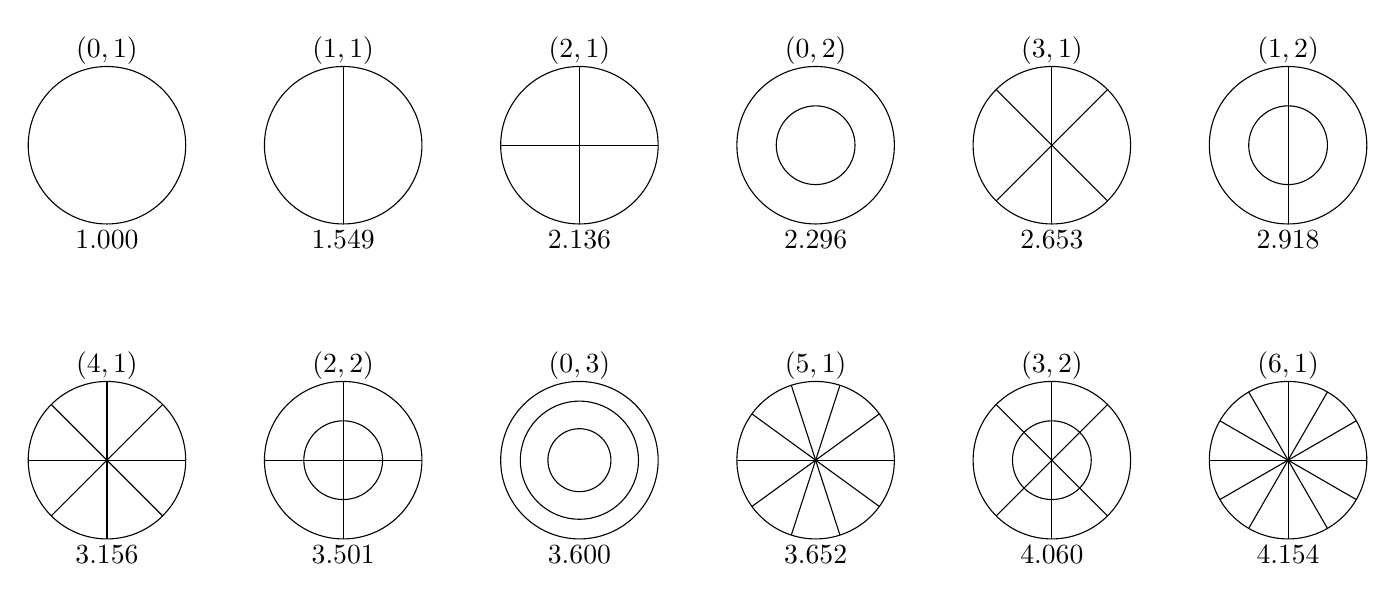
\begin{tikzpicture}
    \foreach \x in {0, 3, 6, 9, 12, 15}
        {\draw (\x, 0) circle (1cm);
        \draw (\x, -4) circle (1cm);
    }

    %Primera línea de modos normales de vibración
    \node at (0, 1.2) {$(0, 1)$};
    \node at (3, 1.2) {$(1, 1)$};
    \node at (6, 1.2) {$(2, 1)$};
    \node at (9, 1.2) {$(0, 2)$};
    \node at (12, 1.2) {$(3, 1)$};
    \node at (15, 1.2) {$(1, 2)$};

    %frecuencia
    \node at (0, -1.2) {$1.000$};
    \node at (3, -1.2) {$1.549$};
    \node at (6, -1.2) {$2.136$};
    \node at (9, -1.2) {$2.296$};
    \node at (12, -1.2) {$2.653$};
    \node at (15, -1.2) {$2.918$};

    %(1, 1)
    \draw (3, -1) -- (3, 1);
    
    %(2, 1)
    \draw (6, -1) -- (6, 1);
    \draw (5, 0) -- (7, 0);

    %(0, 2)
    \draw (9, 0) circle (0.5cm);

    %(3, 1)
    \draw (12, -1) -- (12, 1);
    \draw [rotate around={45:(12,0)}] (11, 0) -- (13, 0);
    \draw [rotate around={-45:(12,0)}] (11, 0) -- (13, 0);
    
    %(1, 2)
    \draw (15, 0) circle (0.5cm);
    \draw (15, -1) -- (15, 1);

    %Segunda línea de modos normales de vibración
    \node at (0, -2.8) {$(4, 1)$};
    \node at (3, -2.8) {$(2, 2)$};
    \node at (6, -2.8) {$(0, 3)$};
    \node at (9, -2.8) {$(5, 1)$};
    \node at (12, -2.8) {$(3, 2)$};
    \node at (15, -2.8) {$(6, 1)$};

    %frecuencias
    \node at (0, -5.2) {$3.156$};
    \node at (3, -5.2) {$3.501$};
    \node at (6, -5.2) {$3.600$};
    \node at (9, -5.2) {$3.652$};
    \node at (12, -5.2) {$4.060$};
    \node at (15, -5.2) {$4.154$};

    %(4, 1)
    \draw (-1, -4) -- (1, -4);
    \draw (0, -5) -- (0, -3);
    \draw [rotate around={45:(0, -4)}] (-1, -4) -- (1, -4);
    \draw [rotate around={-45:(0, -4)}] (-1, -4) -- (1, -4);
    
    %(2, 2)
    \draw (3, -4) circle (0.5cm);
    \draw (2, -4) -- (4, -4);
    \draw (3, -5) -- (3, -3);

    %(0, 3)
    \draw (6, -4) circle (0.75cm);
    \draw (6, -4) circle (0.4cm);

    %(5, 1)
    \draw (8, -4) -- (10, -4); 
    \draw [rotate around={36:(9, -4)}] (8, -4) -- (10, -4);
    \draw [rotate around={72:(9, -4)}] (8, -4) -- (10, -4);
    \draw [rotate around={-36:(9, -4)}] (8, -4) -- (10, -4);
    \draw [rotate around={-72:(9, -4)}] (8, -4) -- (10, -4);

    %(3, 2)
    \draw (12, -4) circle (0.5cm);
    \draw (12, -5) -- (12, -3);
    \draw [rotate around={45:(12, -4)}] (11, -4) -- (13, -4);
    \draw [rotate around={-45:(12, -4)}] (11, -4) -- (13, -4);

    %(6, 1)
    \draw (14, -4) -- (16, -4);
    \draw (15, -5) -- (15, -3);
    \draw [rotate around={30:(15, -4)}] (14, -4) -- (16, -4);
    \draw [rotate around={60:(15, -4)}] (14, -4) -- (16, -4);
    \draw [rotate around={-30:(15, -4)}] (14, -4) -- (16, -4);
    \draw [rotate around={-60:(15, -4)}] (14, -4) -- (16, -4);


\end{tikzpicture}
\end{document}